% Παράρτημα A

\chapter{Datasets Structure \& Analysis}


%========================================
%========================================
%========================================
\section{Business Entries Dataset}

This appendix contains information about the business dataset after unifying the entries from multiple sources, filling the missing values, and adding the NACE code:

%========================================
%========================================
\subsection{Dataset Structure}

This section provides the structure of the pure business dataset (before joining).

\begin{longtable}{p{5cm} p{10cm}}
    \caption{Business Dataset Columns (highlighted features are used for joining)} \label{tab:business_columns} \\
    \hline
    \textbf{Column Name} & \textbf{Description} \\
    \hline
    \endfirsthead
    
    \multicolumn{2}{c}{{\bfseries Table \thetable\ (continued)}} \\
    \hline
    \textbf{Column Name} & \textbf{Description} \\
    \hline
    \endhead
    
    \hline \multicolumn{2}{r}{{Continued on next page}} \\
    \endfoot
    
    \hline
    \endlastfoot
    
    Name & Business name as listed in the source dataset \\
    Category & General business category (e.g., restaurant, retail, service) \\
    Latitude & Geographic latitude coordinate of the business location \\
    Longitude & Geographic longitude coordinate of the business location \\
    Address & Full street address of the business \\
    Country & Country where the business is located \\
    City & City where the business is located \\
    Postal Code & Postal code of the business location \\
    Rating & Average rating score given by customers, if available \\
    Reviews & Number of customer reviews, if available \\
    Source & Origin of the business entry \\
    Description & Short textual description of the business \\
    NACE Code & Official NACE classification code for the business activity \\
    NACE Description (EN) & English description of the NACE code activity \\
    \rowcolor{yellow!20}
    Municipal Community & The municipal community of the business location\\
    \rowcolor{yellow!20}
    Neighborhood & The neighborhood of the business location\\
    
\end{longtable}

%========================================
%========================================
\subsection{Dataset Analysis}


\subsubsection{Feature Values Distributions}

Here we see the most frequent values of the business dataset features that were not explicitly mentioned in the paragraph \ref{EDA_business}.

\begin{figure}[h]
    \centering
    \begin{minipage}[b]{0.45\textwidth}
        \centering
        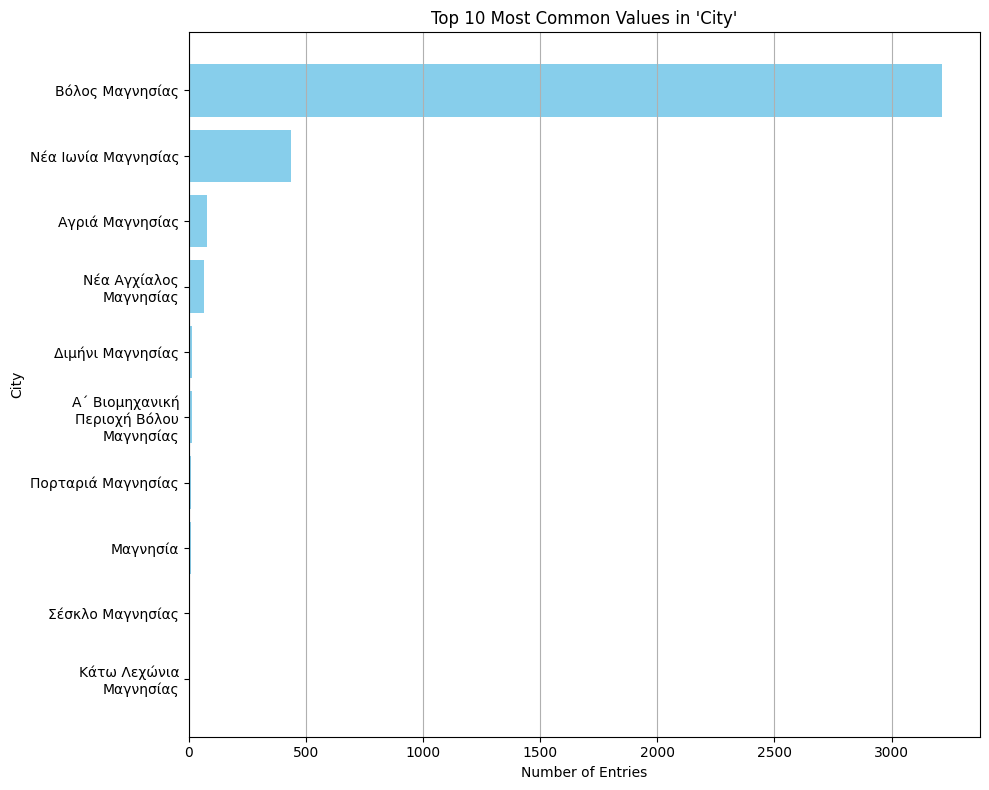
\includegraphics[height=5cm]{figures/distribution_city.png}
        \caption{'City' Bar Chart}
        \label{fig:city_distr}
    \end{minipage}
    \hfill
    \begin{minipage}[b]{0.45\textwidth}
        \centering
        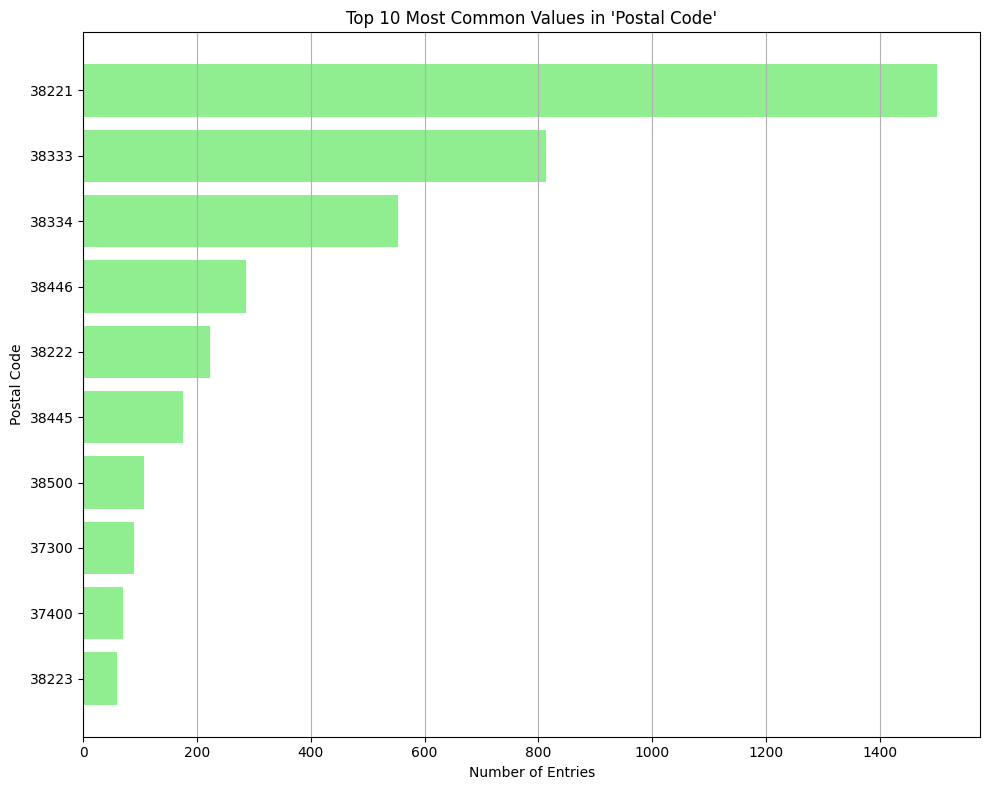
\includegraphics[height=5cm]{figures/distribution_postal_code.png}
        \caption{'Postal Code' Bar Chart}
        \label{fig:postal_distr}
    \end{minipage}
\end{figure}

\begin{figure}[h]
    \centering
    \begin{minipage}[b]{0.45\textwidth}
        \centering
        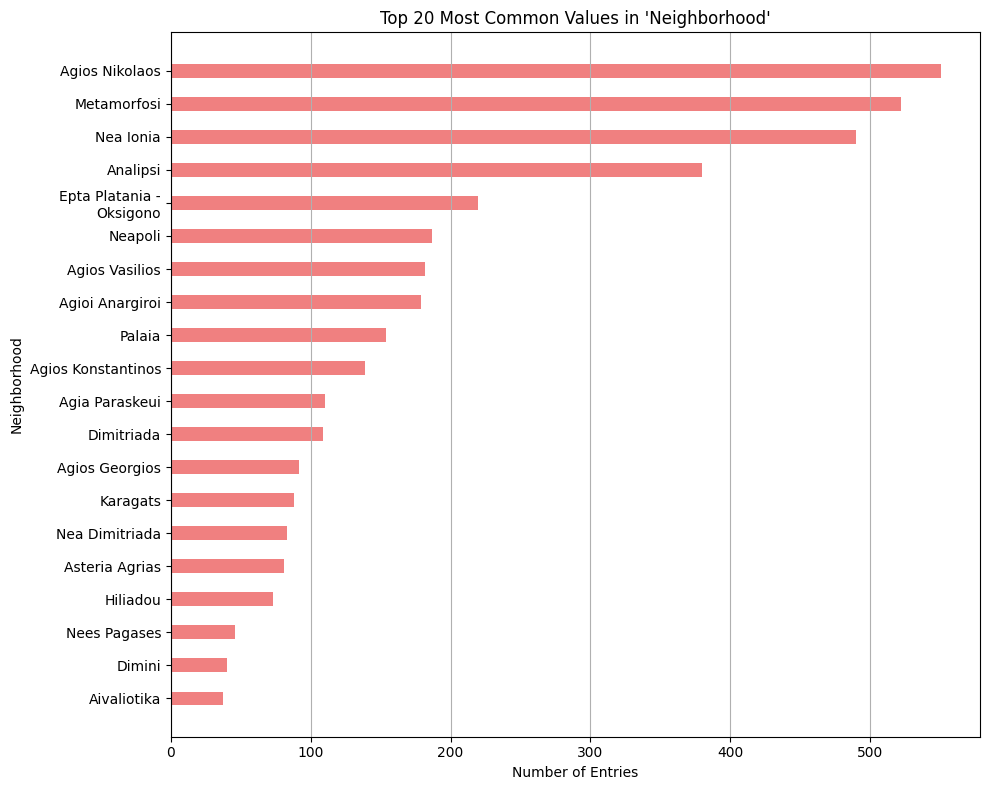
\includegraphics[height=5cm]{figures/distribution_neighborhoods.png}
        \caption{'Neighborhood' Bar Chart}
        \label{fig:neighborhood_distr}
    \end{minipage}
    \hfill
    \begin{minipage}[b]{0.45\textwidth}
        \centering
        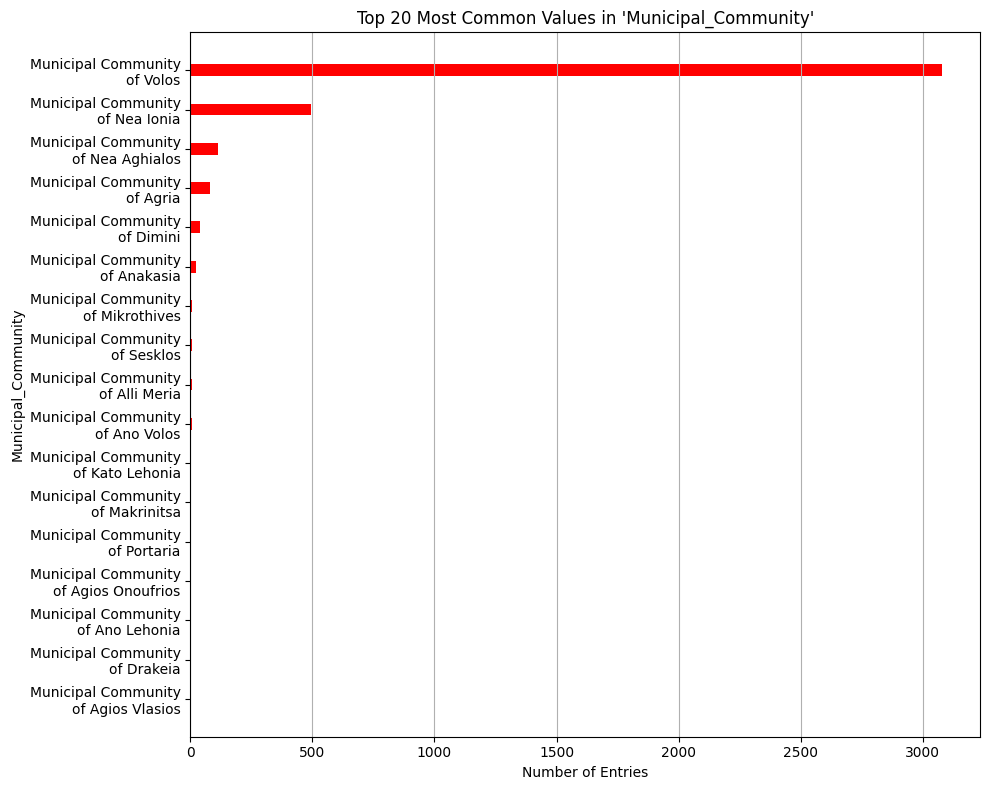
\includegraphics[height=5cm]{figures/distribution_mc.png}
        \caption{'MC' Bar Chart}
        \label{fig:mc_distr}
    \end{minipage}
\end{figure}

\begin{figure}[h]
    \centering
    \begin{minipage}[b]{0.45\textwidth}
        \centering
        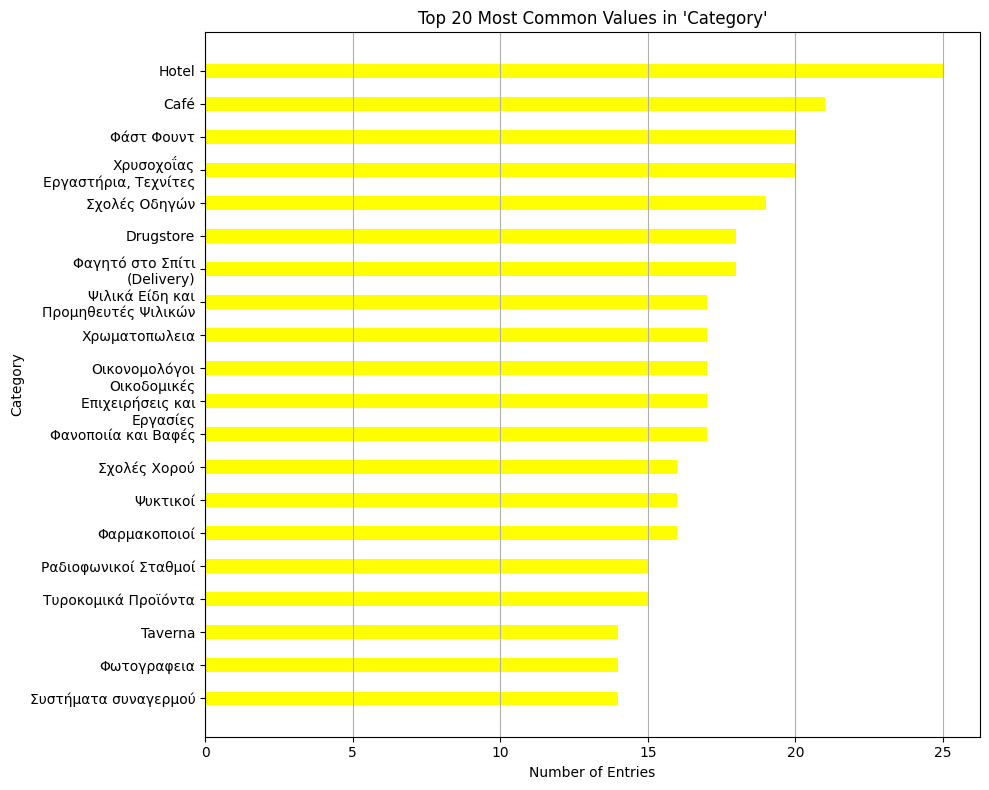
\includegraphics[height=5cm]{figures/distribution_category.png}
        \caption{'Category' Bar Chart}
        \label{fig:category_distr}
    \end{minipage}
    \hfill
    \begin{minipage}[b]{0.45\textwidth}
        \centering
        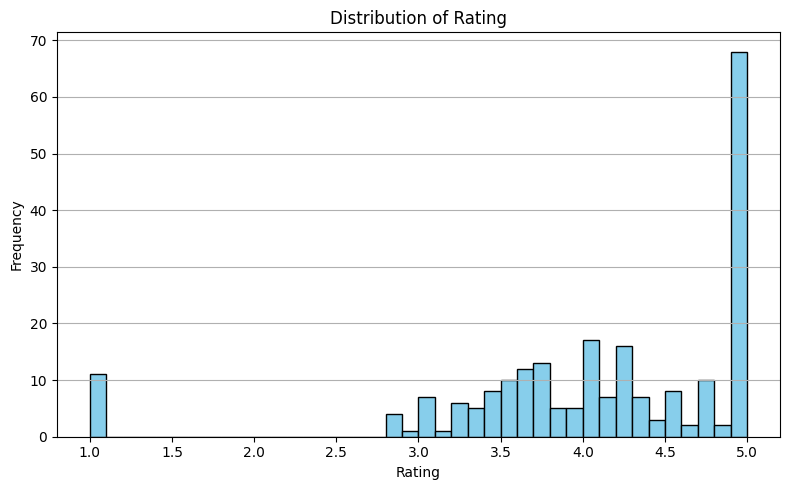
\includegraphics[height=5cm]{figures/distribution_rating.png}
        \caption{'Rating' Histogram}
        \label{fig:distr_rating}
    \end{minipage}
\end{figure}



%========================================
%========================================
%========================================
\newpage
\section{ELSTAT Datasets}

This appendix contains information about the data extracted from the ELSTAT platform: their raw structure, visualizations about their analysis, and more.

%========================================
%========================================
\subsection{Datasets Structure}

Here we present the complete structure of the raw demographic and economic data extracted from the ELSTAT platform.


%========================================
\subsubsection{Raw Demographic Data}

\begin{longtable}{p{5cm} p{10cm}}
    \caption{Demographic Dataset Columns} \label{tab:demographic_columns} \\
    \hline
    \textbf{Column Name} & \textbf{Description} \\
    \hline
    \endfirsthead
    
    \multicolumn{2}{c}{{\bfseries Table \thetable\ (continued)}} \\
    \hline
    \textbf{Column Name} & \textbf{Description} \\
    \hline
    \endhead
    
    \hline \multicolumn{2}{r}{{Continued on next page}} \\
    \endfoot
    
    \hline
    \endlastfoot
    
    ΠΕΡΙΦΕΡΕΙΑΚΗ ΕΝΟΤΗΤΑ & Administrative regional unit where the municipal community belongs \\
    ΔΗΜΟΣ & Municipality name \\
    ΔΗΜΟΤΙΚΗ ΕΝΟΤΗΤΑ & Administrative municipal unit \\
    ΔΗΜΟΤΙΚΗ ΚΟΙΝΟΤΗΤΑ & Administrative municipal community name (Greek) \\
    Population & Total population count \\
    0-4 & Population aged 0 to 4 years \\
    5-9 & Population aged 5 to 9 years \\
    10-14 & Population aged 10 to 14 years \\
    15-19 & Population aged 15 to 19 years \\
    20-24 & Population aged 20 to 24 years \\
    25-29 & Population aged 25 to 29 years \\
    30-34 & Population aged 30 to 34 years \\
    35-39 & Population aged 35 to 39 years \\
    40-44 & Population aged 40 to 44 years \\
    45-49 & Population aged 45 to 49 years \\
    50-54 & Population aged 50 to 54 years \\
    55-59 & Population aged 55 to 59 years \\
    60-64 & Population aged 60 to 64 years \\
    65-69 & Population aged 65 to 69 years \\
    70-74 & Population aged 70 to 74 years \\
    75+ & Population aged 75 years and older \\
    higher\_education & Individuals with higher education (university or equivalent) \\
    post\_secondary\_non\_uni & Individuals with post-secondary non-university education \\
    high\_school & Individuals with completed high school education \\
    lower\_secondary & Individuals with completed lower secondary education \\
    primary\_education & Individuals with completed primary education \\
    no\_formal\_education & Individuals with no formal education \\
    not\_classified & Individuals whose education level is not classified \\
    Άγαμοι & Individuals who are unmarried \\
    Έγγαμοι & Individuals who are married \\
    Χήροι & Individuals who are widowed \\
    Διαζευγμένοι & Individuals who are divorced \\
\end{longtable}


%========================================
\newpage
\subsubsection{Raw Economic Data}

\begin{longtable}{p{5cm} p{10cm}}
    \caption{Economic Dataset Columns} \label{tab:economic_columns} \\
    \hline
    \textbf{Column Name} & \textbf{Description} \\
    \hline
    \endfirsthead
    
    \multicolumn{2}{c}{{\bfseries Table \thetable\ (continued)}} \\
    \hline
    \textbf{Column Name} & \textbf{Description} \\
    \hline
    \endhead
    
    \hline \multicolumn{2}{r}{{Continued on next page}} \\
    \endfoot
    
    \hline
    \endlastfoot
    
    ΠΕΡΙΦΕΡΕΙΑΚΗ ΕΝΟΤΗΤΑ & Administrative regional unit where the municipal community belongs \\
    ΔΗΜΟΣ & Municipality name \\
    ΔΗΜΟΤΙΚΗ ΕΝΟΤΗΤΑ & Administrative municipal unit \\
    ΔΗΜΟΤΙΚΗ ΚΟΙΝΟΤΗΤΑ & Administrative municipal community name (Greek) \\
    Σύνολο & Total reference population for the economic activity statistics \\
    Οικονομικά ενεργοί & Economically active population (employed + unemployed individuals) \\
    Απασχολούμενοι & Employed individuals within the economically active population \\
    Πρωτογενής & Number of employed individuals in the primary economic sector \\
    Δευτερογενής & Number of employed individuals in the secondary economic sector \\
    Τριτογενής & Number of employed individuals in the tertiary economic sector \\
    Άνεργοι & Unemployed individuals within the economically active population \\
    Οικονομικά μη ενεργοί & Economically inactive population (students, retirees, homemakers, etc.) \\
\end{longtable}


%========================================
\newpage
\subsubsection{Processed Demographic \& Economic Data}

\begin{longtable}{p{5cm} p{10cm}}
    \caption{Processed Demographic \& Economic Dataset Columns} \label{tab:final_municipal_communities_columns} \\
    \hline
    \textbf{Column Name} & \textbf{Description} \\
    \hline
    \endfirsthead
    
    \multicolumn{2}{c}{{\bfseries Table \thetable\ (continued)}} \\
    \hline
    \textbf{Column Name} & \textbf{Description} \\
    \hline
    \endhead
    
    \hline \multicolumn{2}{r}{{Continued on next page}} \\
    \endfoot
    
    \hline
    \endlastfoot
    
    ΠΕΡΙΦΕΡΕΙΑΚΗ ΕΝΟΤΗΤΑ & Administrative regional unit where the municipal community belongs \\
    ΔΗΜΟΣ & Municipality name \\
    ΔΗΜΟΤΙΚΗ ΕΝΟΤΗΤΑ & Administrative municipal unit \\
    ΔΗΜΟΤΙΚΗ ΚΟΙΝΟΤΗΤΑ ΕΛΛ & Municipal community name in Greek \\
    ΔΗΜΟΤΙΚΗ ΚΟΙΝΟΤΗΤΑ & Municipal community name in English \\
    Population & Total population count \\
    Άγαμοι\_pct & Percentage of unmarried individuals \\
    Έγγαμοι\_pct & Percentage of married individuals \\
    Χήροι\_pct & Percentage of widowed individuals \\
    Διαζευγμένοι\_pct & Percentage of divorced individuals \\
    age\_0\_14\_pct & Percentage of population aged 0–14 years \\
    age\_15\_64\_pct & Percentage of population aged 15–64 years \\
    age\_65\_plus\_pct & Percentage of population aged 65 years and older \\
    low\_education\_pct & Percentage of population with no formal, primary, or lower secondary education \\
    medium\_education\_pct & Percentage of population with upper secondary or post-secondary non-university education \\
    high\_education\_pct & Percentage of population with higher education (university or equivalent) \\
    unemployment\_rate & Ratio of unemployed individuals to economically active population \\
    labor\_force\_participation\_rate & Ratio of economically active population to total population \\
    primary\_sector\_pct & Percentage of employed individuals in the primary sector \\
    secondary\_sector\_pct & Percentage of employed individuals in the secondary sector \\
    tertiary\_sector\_pct & Percentage of employed individuals in the tertiary sector \\
    Area\_km2 & Area of the municipal community in square kilometers \\
\end{longtable}


%========================================
%========================================
\subsection{Datasets Analysis}


Here, we present the visualizations provided by analyzing the demographic and economic data gathered from the ELSTAT platform. The results of these inspections led to the chosen transformation methods applied in order to prepare the data for later use.


%========================================
\subsubsection{Feature Values Distributions}

Below, we see the most frequent values of the ELSTAT dataset features that were not explicitly mentioned in the paragraph \ref{EDA_mc}.


\begin{figure}[!htbp]
    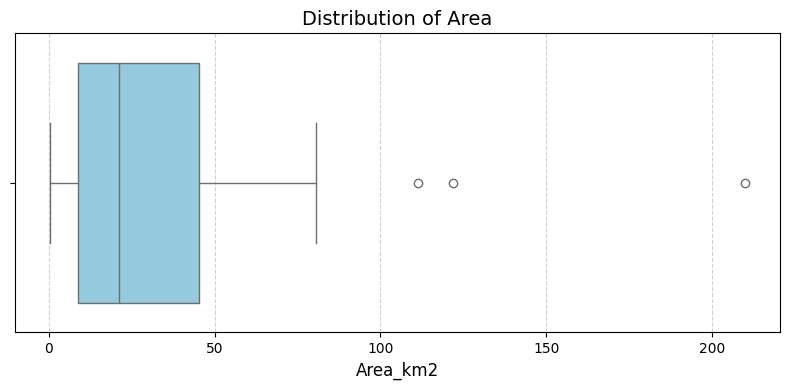
\includegraphics[scale=0.5]{figures/boxplot_area.png}
    \centering
    \caption{'Area\_km2' Feature Boxplot}
    \label{fig:box_area}
\end{figure}

\begin{figure}[!htbp]
    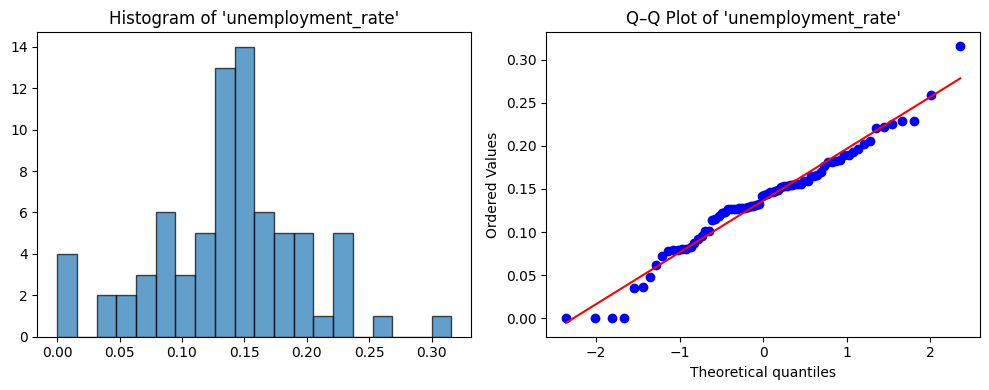
\includegraphics[scale=0.5]{figures/stat_unemployment_rate.png}
    \centering
    \caption{'unemployment\_rate' Feature Histogram \& QQ-Plot}
    \label{fig:stat_unemployment}
\end{figure}

\begin{figure}[!htbp]
    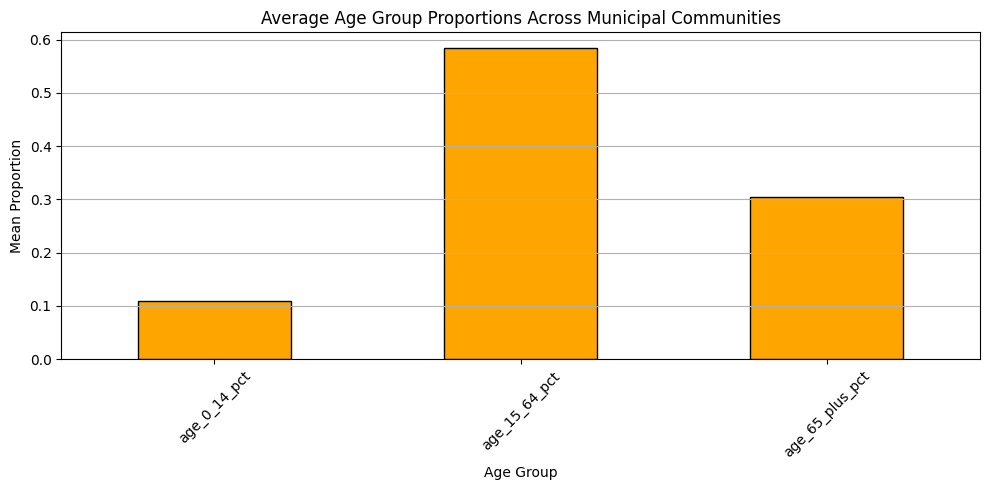
\includegraphics[scale=0.45]{figures/barchart_age_group_means.png}
    \centering
    \caption{Mean Age Group Features Bar Chart}
    \label{fig:bar_age_mean}
\end{figure}

\begin{figure}[!htbp]
    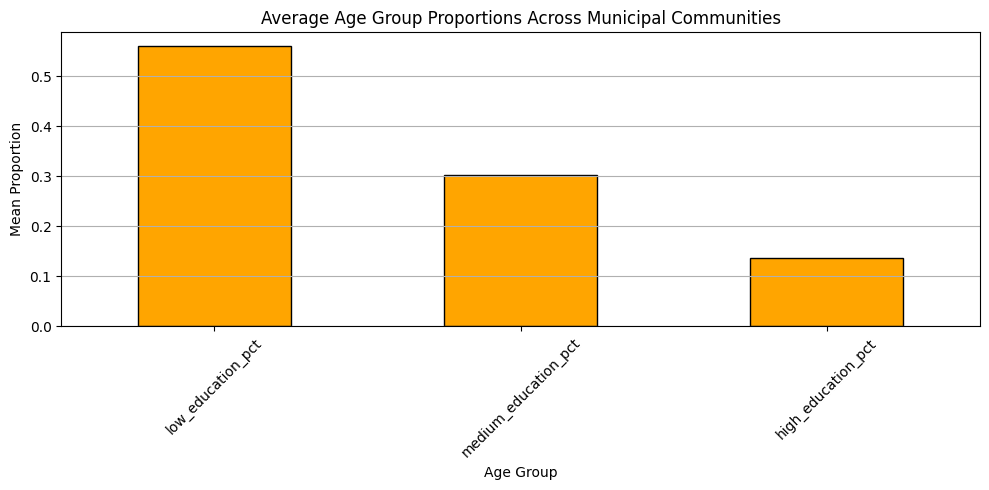
\includegraphics[scale=0.45]{figures/barchart_education_group_means.png}
    \centering
    \caption{Mean Education Group Features Bar Chart}
    \label{fig:bar_education_mean}
\end{figure}

\begin{figure}[!htbp]
    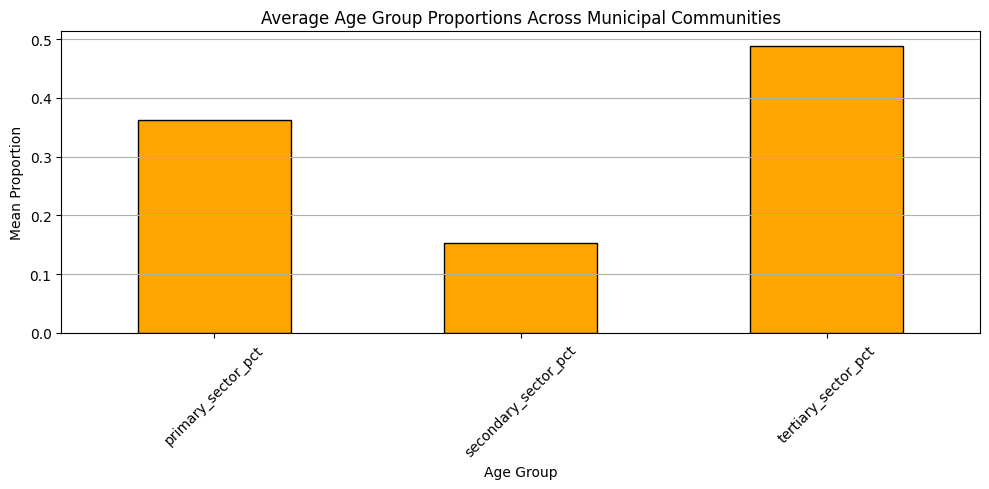
\includegraphics[scale=0.45]{figures/barchart_sector_group_means.png}
    \centering
    \caption{Mean Sector Group Features Bar Chart}
    \label{fig:bar_sector_mean}
\end{figure}


%========================================
\subsubsection{Scatter Plots}

\begin{figure}[h]
    \centering
    \begin{minipage}[b]{0.47\textwidth}
        \centering
        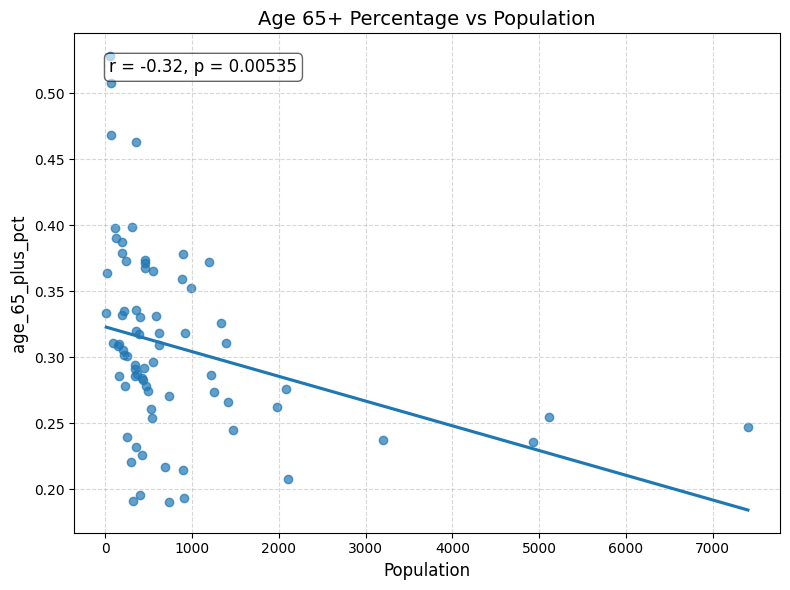
\includegraphics[height=5cm]{figures/scatter_population_elderly.png}
        \caption{Population VS Age 65+}
        \label{fig:scat_pop_elderly}
    \end{minipage}
    \hfill
    \begin{minipage}[b]{0.47\textwidth}
        \centering
        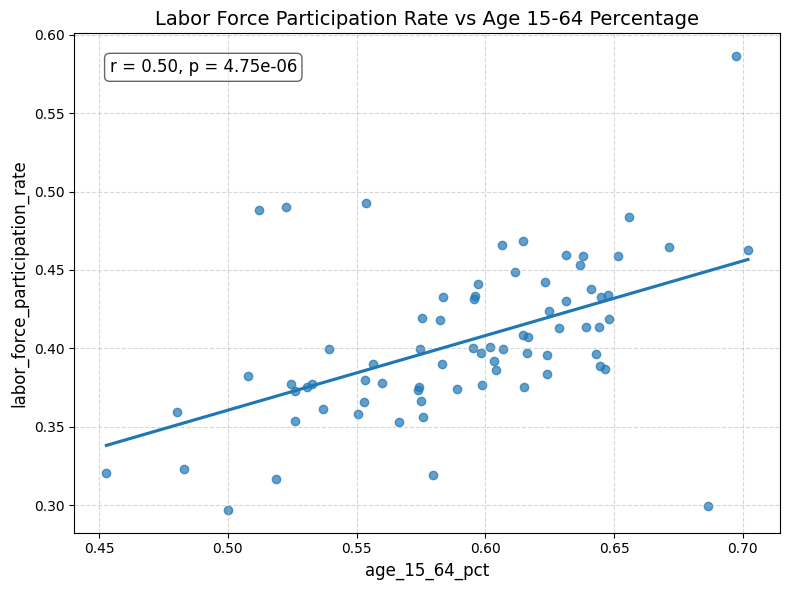
\includegraphics[height=5cm]{figures/scatter_labor_working.png}
        \caption{Labor Force VS Age 15-64 }
        \label{fig:scat_labor_working}
    \end{minipage}
\end{figure}


%========================================
\subsubsection{Correlation Matrices}
\label{sec:correlation_matrices} 

\begin{figure}[!htbp]
    \centering
    \begin{minipage}[b]{0.47\textwidth}
        \centering
        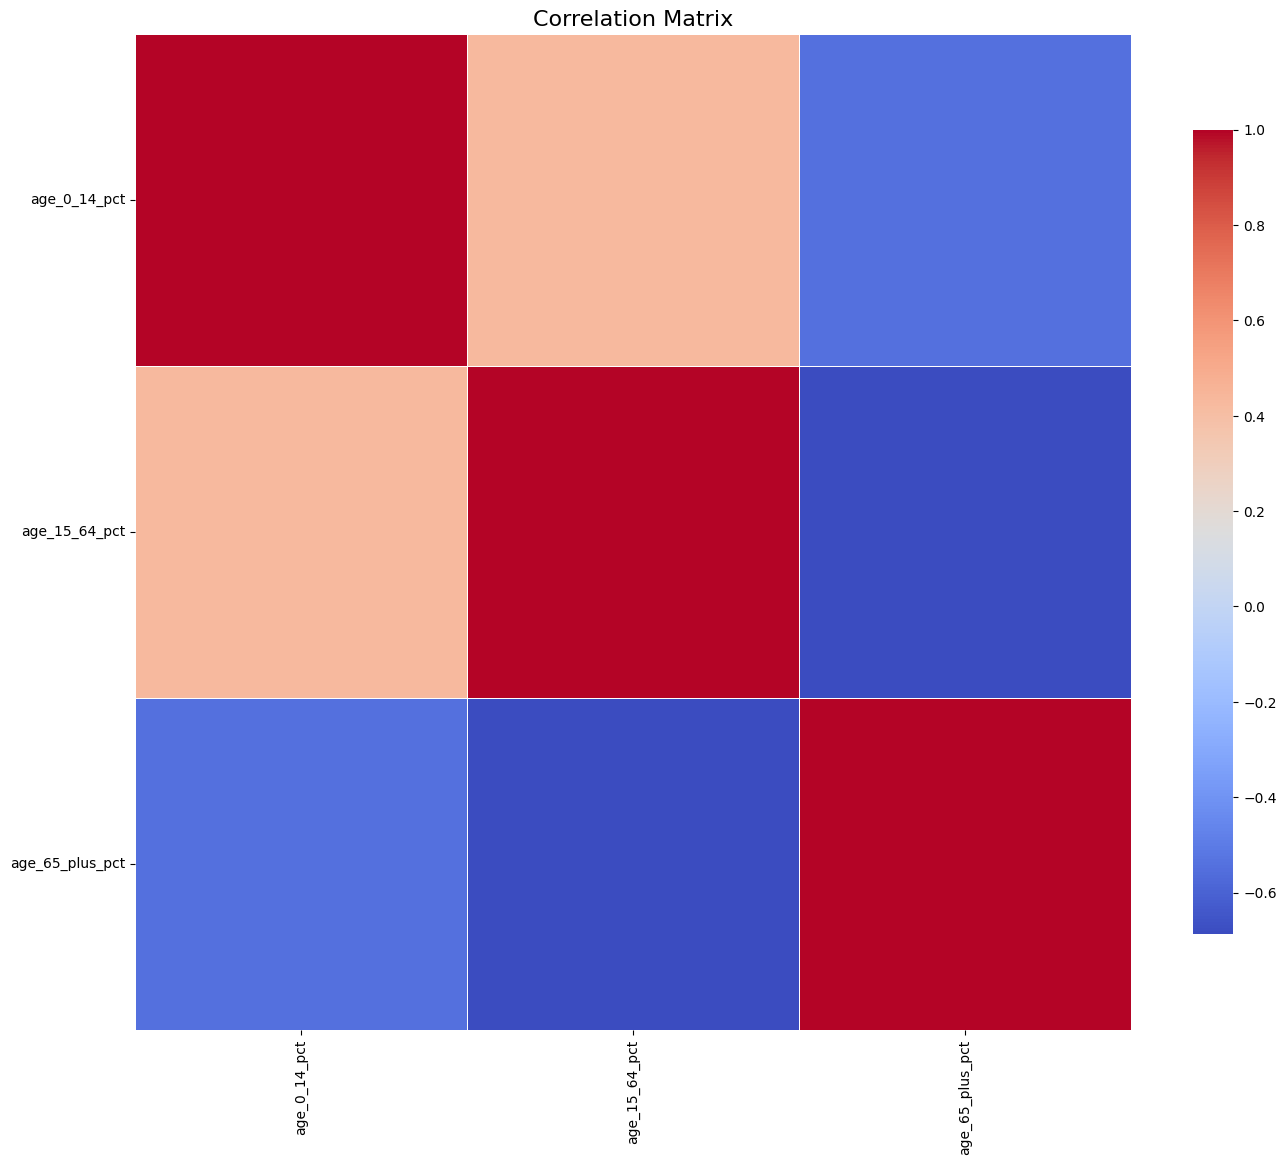
\includegraphics[height=5cm]{figures/corr_age.png}
        \caption{Age Groups}
        \label{fig:corr_age}
    \end{minipage}
    \hfill
    \begin{minipage}[b]{0.47\textwidth}
        \centering
        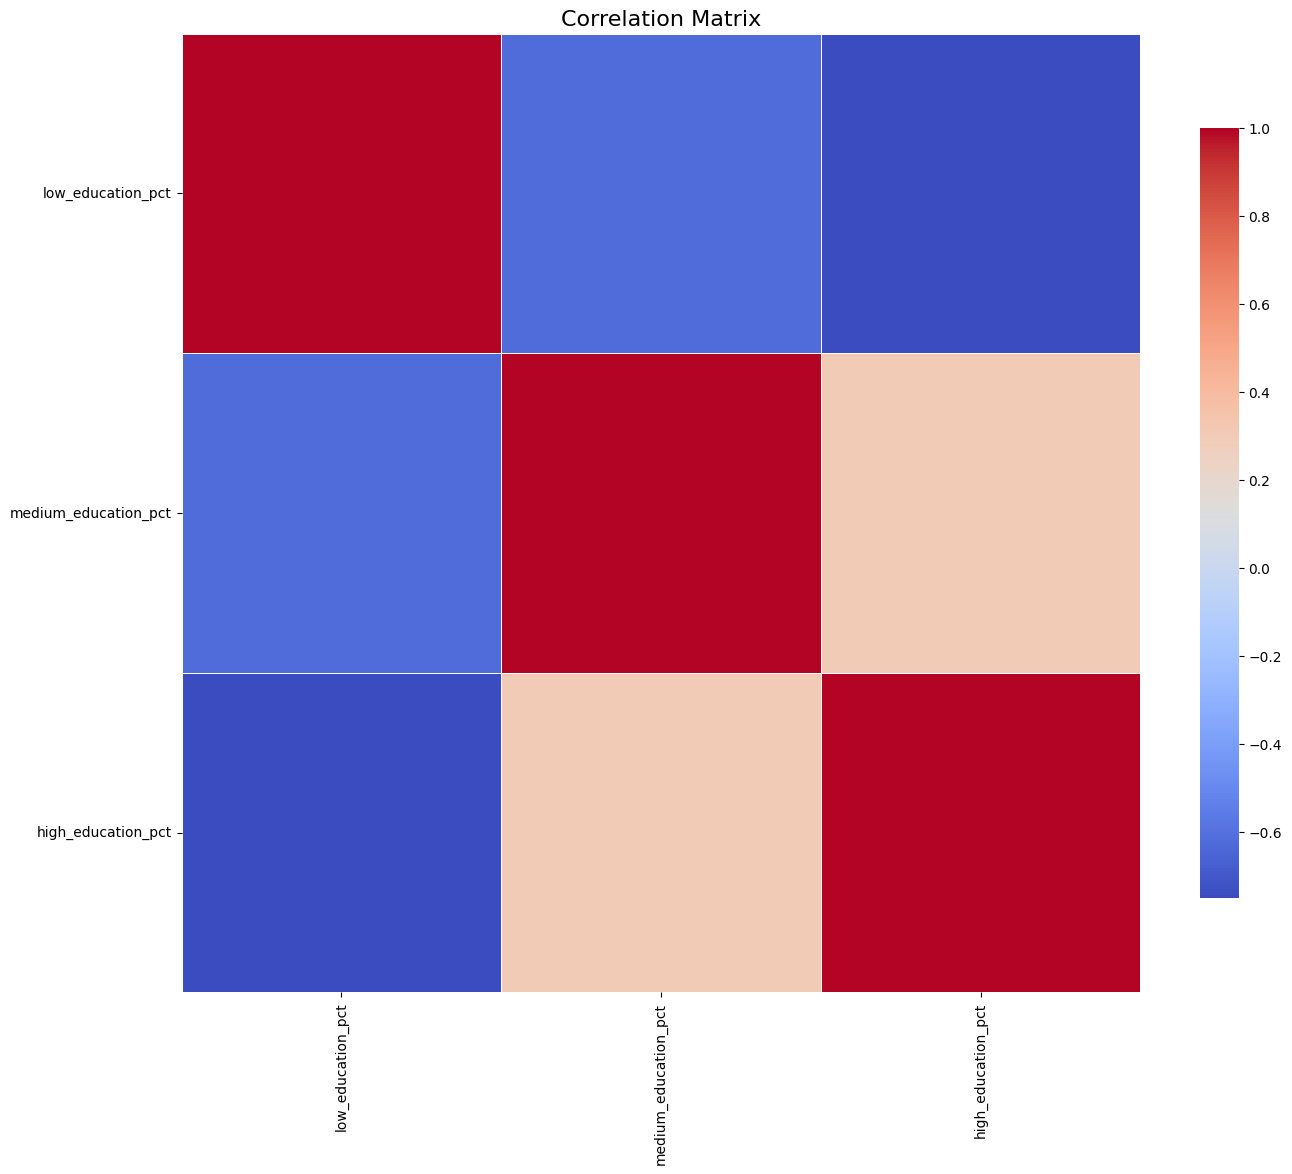
\includegraphics[height=5cm]{figures/corr_education.png}
        \caption{Educational Level Groups}
        \label{fig:corr_education}
    \end{minipage}
\end{figure}

\begin{figure}[!htbp]
    \centering
    \begin{minipage}[b]{0.47\textwidth}
        \centering
        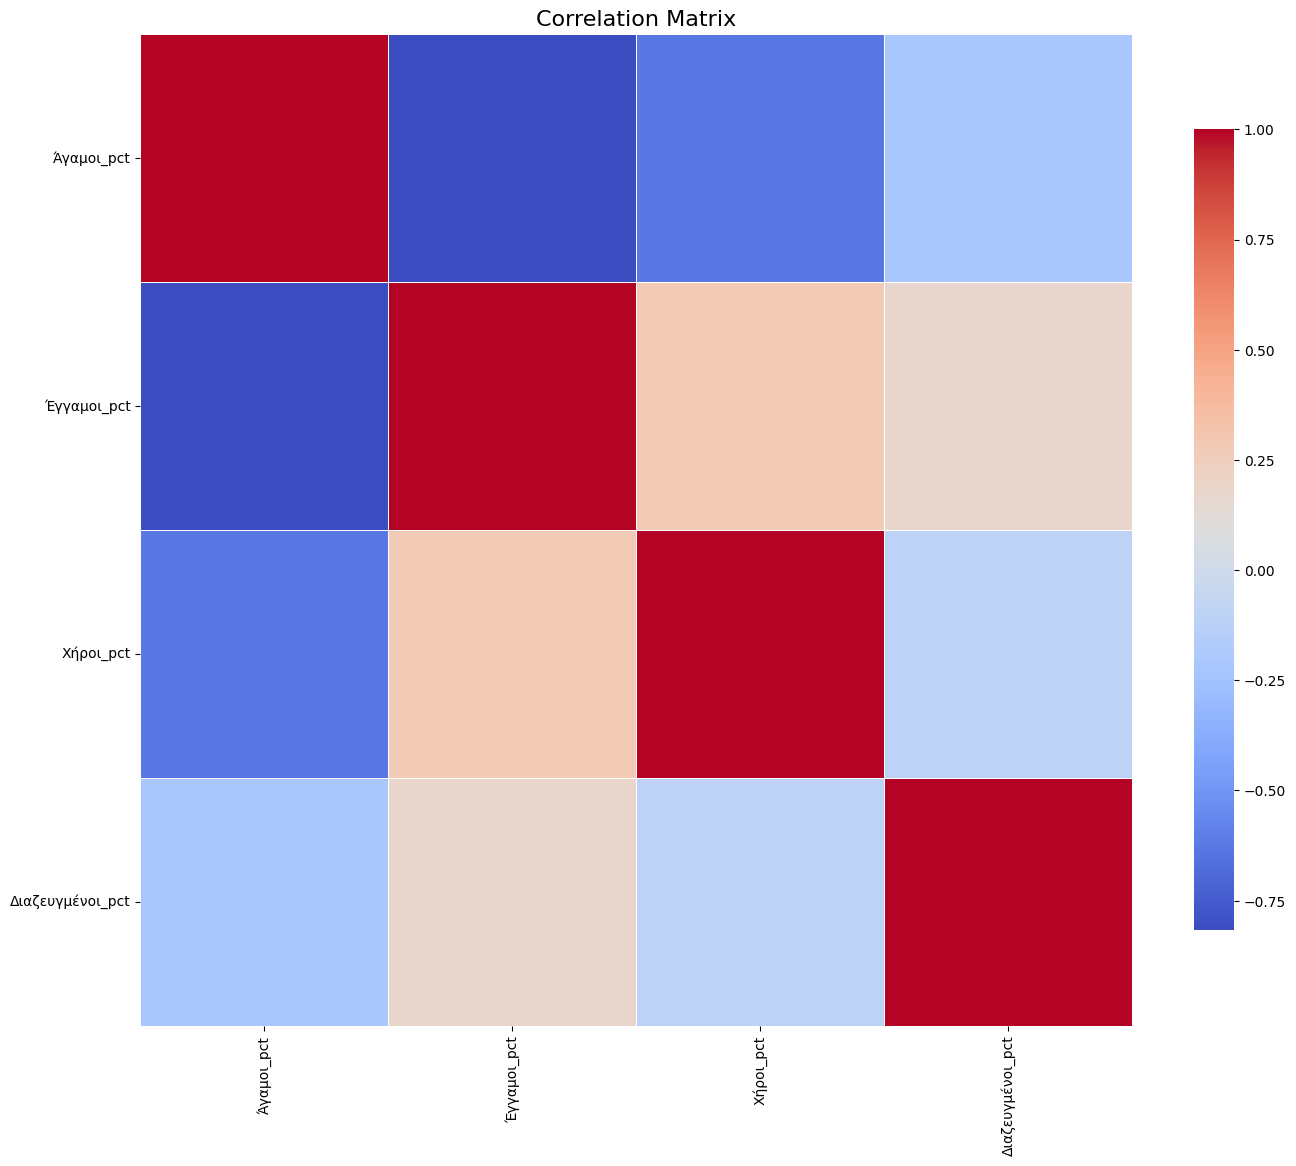
\includegraphics[height=5cm]{figures/corr_marriage.png}
        \caption{Martial Status Groups}
        \label{fig:corr_marriage}
    \end{minipage}
    \hfill
    \begin{minipage}[b]{0.47\textwidth}
        \centering
        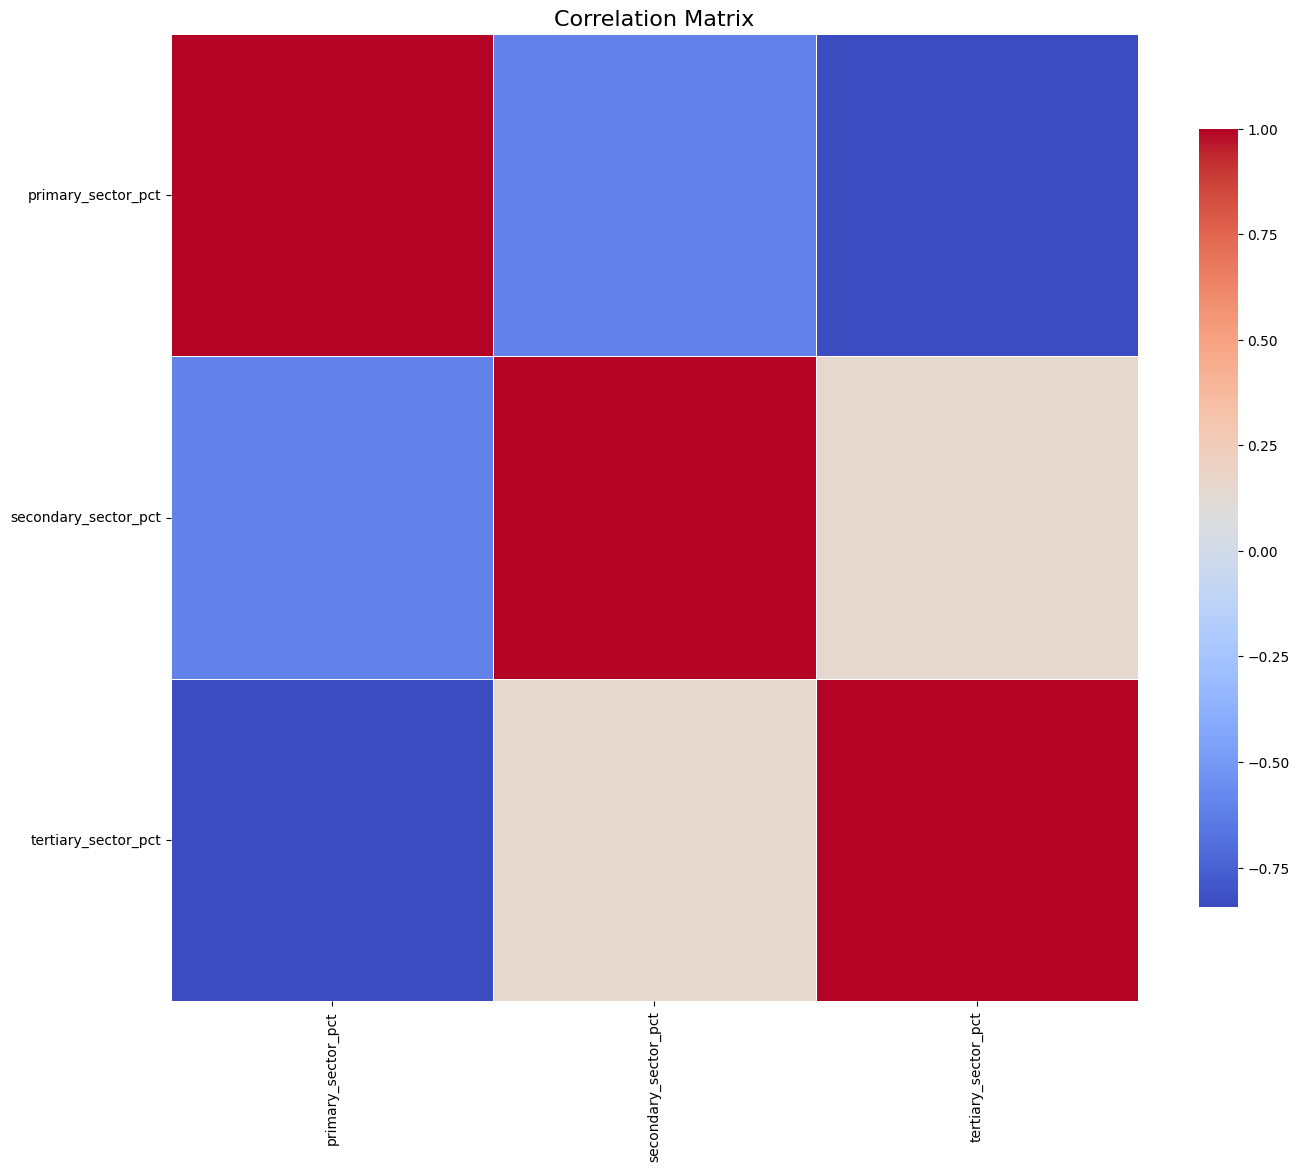
\includegraphics[height=5cm]{figures/corr_sector.png}
        \caption{Sector Groups}
        \label{fig:corr_sector}
    \end{minipage}
\end{figure}


%========================================
\subsubsection{Feature Engineering}
\label{sec:elstat_feature_engineering}

Below is presented the specific modifications performed in the feature groups in order to reduce the dimensionality:

\begin{itemize}
    \item Age Groups: 
        \begin{itemize}
            \item $age\_0\_14\_pct = (0-4)_{\%} + (5-9)_{\%} + (10-14)_{\%}$ (younger people)
            \item $age\_15\_64\_pct = (15-19)_{\%} + (20-24)_{\%} + (25-29)_{\%} + (30-34)_{\%} + (35-39)_{\%} + (40-44)_{\%} + (45-49)_{\%} + (50-54)_{\%} + (55-59)_{\%} + (60-64)_{\%}$ (working people)
            \item $age\_65\_plus\_pct = (65-69)_{\%} + (70-74)_{\%} + (75+)_{\%}$ (elderly people)
        \end{itemize}

    \item Educational Level Groups:
        \begin{itemize}
            \item $low\_education\_pct = no\_formal\_education_{\%} + primary\_education_{\%} + lower\_secondary_{\%}$
            \item $medium\_education\_pct = high\_school_{\%} + post\_secondary\_non\_uni_{\%}$
            \item $high\_education\_pct = higher\_education_{\%}$
        \end{itemize}

    \item Economic Hierarchical Features:
        \begin{itemize}
            \item $unemployment\_rate = \frac{\text{Άνεργοι}}{\text{Οικονομικά ενεργοί}}$
            \item $labor\_force\_participation\_rate = \frac{\text{Οικονομικά ενεργοί}}{\text{Σύνολο}}$
            \item $primary\_sector\_pct = \frac{\text{Πρωτογενής}}{\text{Απασχολούμενοι}}$
            \item $secondary\_sector\_pct = \frac{\text{Δευτερογενής}}{\text{Απασχολούμενοι}}$
            \item $tertiary\_sector\_pct = \frac{\text{Τριτογενής}}{\text{Απασχολούμενοι}}$
        \end{itemize}
\end{itemize}




%========================================
%========================================
%========================================

\section{Neighborhoods Dataset}

This section provides information about the structure of the Neighborhoods Dataset after extracting additional features from QGIS:


%========================================
\subsection{Datasets Structure}

Here we present the structure of the neighborhood dataset. 

\begin{longtable}{p{5cm} p{10cm}}
    \caption{Neighborhood Dataset Columns (highlighted features are used for joining)} \label{tab:neighborhood_columns} \\
    \hline
    \textbf{Column Name} & \textbf{Description} \\
    \hline
    \endfirsthead
    
    \multicolumn{2}{c}{{\bfseries Table \thetable\ (continued)}} \\
    \hline
    \textbf{Column Name} & \textbf{Description} \\
    \hline
    \endhead
    
    \hline \multicolumn{2}{r}{{Continued on next page}} \\
    \endfoot
    
    \hline
    \endlastfoot
    
    Neighborhood\_Greek & Neighborhood name in Greek \\
    Neighborhood & Neighborhood name in English \\
    Centroid\_x & Longitude coordinate of the neighborhood centroid \\
    Centroid\_y & Latitude coordinate of the neighborhood centroid \\
    Neighborhood\_Area\_km2 & Total area of the neighborhood polygon in square kilometers \\
    Geometry & Polygon geometry representing the neighborhood boundary \\
    distance\_to\_volos\_center\_km & Distance from the neighborhood centroid to the Volos city center (km)\\
    distance\_to\_volos\_port\_km & Distance from the neighborhood centroid to the Volos port (km)\\
    dist\_to\_main\_road\_km & Distance from the neighborhood centroid to the nearest main road (km)\\
    dist\_to\_bus\_stop\_km & Distance from the neighborhood centroid to the nearest bus stop (km)\\
    dist\_to\_university\_km & Distance from the neighborhood centroid to the University of Thessaly (km)\\
    \rowcolor{yellow!20}
    Municipal Community & Administrative municipal community in which the neighborhood is located \\
\end{longtable}



%========================================
%========================================
\subsection{Dataset Analysis}

Below we show various visualizations that occured during the EDA of the neighborhood dataset.

%========================================

\subsubsection{Feature Values Distributions}
\FloatBarrier

\begin{figure}[!htbp]
    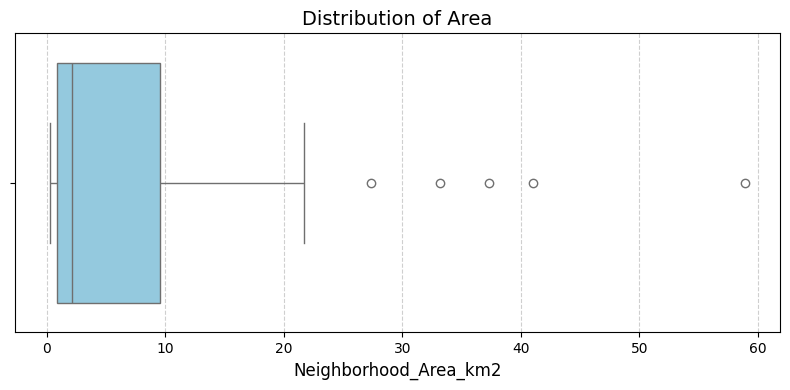
\includegraphics[scale=0.5]{figures/boxplot_area_neighbor.png}
    \centering
    \caption{'Neighborhood\_area\_km2' Feature Boxplot}
    \label{fig:box_area_neigh}
\end{figure}

\begin{figure}[!htbp]
    \centering
    \begin{subfigure}[b]{0.47\textwidth}
        \centering
        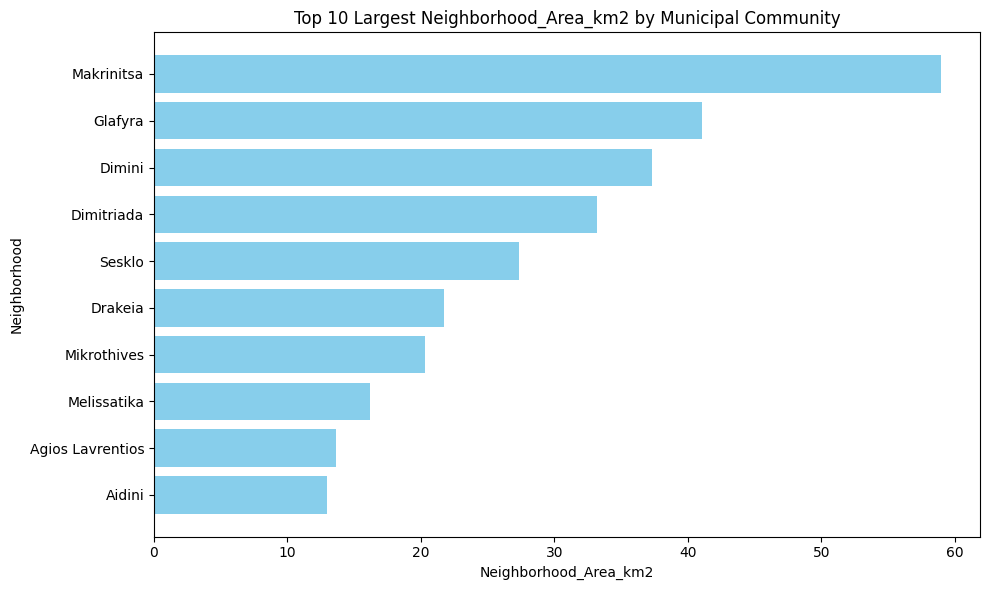
\includegraphics[height=5cm]{figures/barchart_area_neighborhood.png}
        \caption{Neighborhood area Bar Chart}
        \label{fig:bar_area_neigh}
    \end{subfigure}
    \hfill
    \begin{subfigure}[b]{0.47\textwidth}
        \centering
        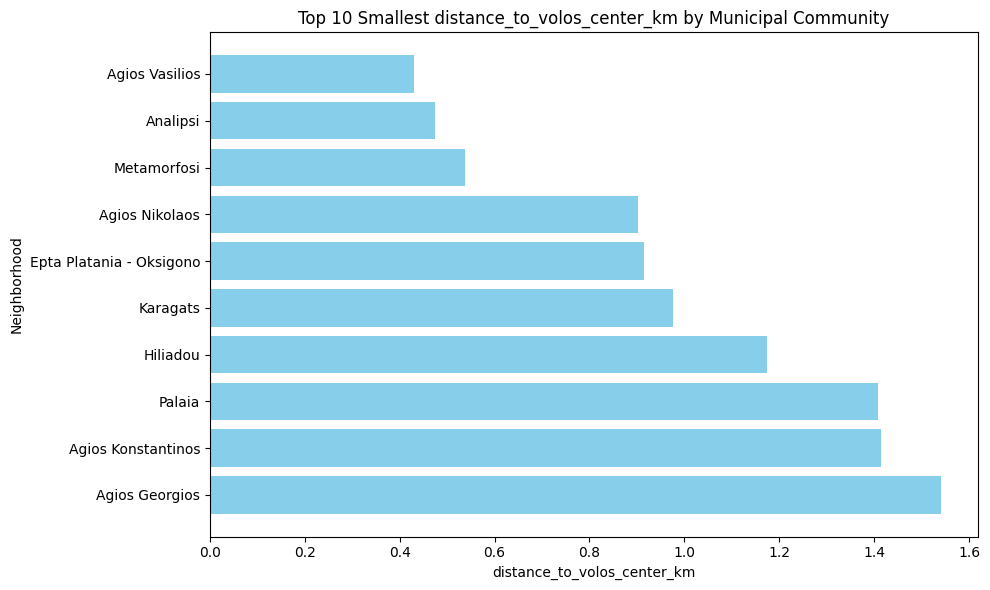
\includegraphics[height=5cm]{figures/barchart_center.png}
        \caption{'Distance to Center  Bar Chart}
        \label{fig:bar_center_neigh}
    \end{subfigure}
\end{figure}

%========================================
\newpage
\subsubsection{Scatter Plots}
\FloatBarrier

\begin{figure}[!htbp]
    \centering
    \begin{subfigure}[b]{0.47\textwidth}
        \centering
        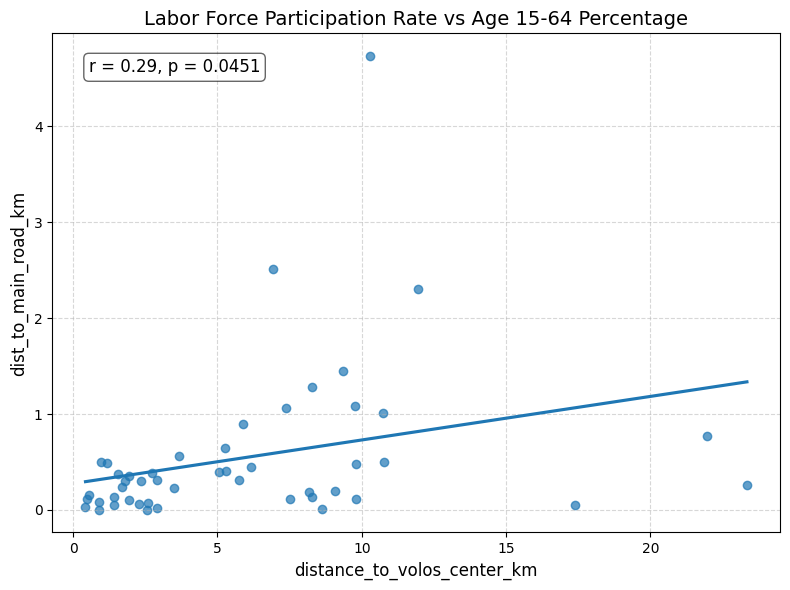
\includegraphics[height=5cm]{figures/scatter_center_highway.png}
        \caption{Distance from Center VS Distance from Main Roads}
        \label{fig:scatter_center_highway}
    \end{subfigure}
    \hfill
    \begin{subfigure}[b]{0.47\textwidth}
        \centering
        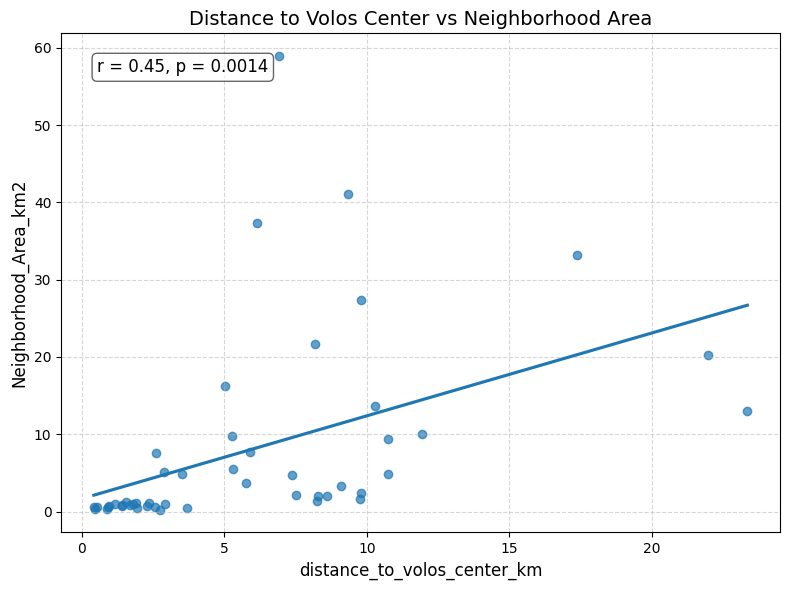
\includegraphics[height=5cm]{figures/scatter_center_area.png}
        \caption{Distance from Center VS Neighborhood Area}
        \label{fig:scatter_center_area}
    \end{subfigure}
\end{figure}





%========================================
%========================================
%========================================
\section{Joined Dataset}

This appendix contains information about the business dataset after joining it both with the neighborhood and municipal community features. 

%========================================
%========================================
\subsection{Dataset Structure}

This section provides the structure of the joined business dataset.

\begin{longtable}{p{5cm} p{10cm}}
    \caption{Joined Dataset Columns} \label{tab:business_joined_columns} \\
    \hline
    \textbf{Column Name} & \textbf{Description} \\
    \hline
    \endfirsthead
    
    \multicolumn{2}{c}{{\bfseries Table \thetable\ (continued)}} \\
    \hline
    \textbf{Column Name} & \textbf{Description} \\
    \hline
    \endhead
    
    \hline \multicolumn{2}{r}{{Continued on next page}} \\
    \endfoot
    
    \hline
    \endlastfoot
    
    Name & Business name as listed in the source dataset \\
    Category & General business category (e.g., restaurant, retail, service) \\
    Latitude & Geographic latitude coordinate of the business location \\
    Longitude & Geographic longitude coordinate of the business location \\
    Address & Full street address of the business \\
    Country & Country where the business is located \\
    City & City where the business is located \\
    Postal Code & Postal code of the business location \\
    Rating & Average rating score given by customers, if available \\
    Reviews & Number of customer reviews, if available \\
    Source & Origin of the business entry \\
    Description & Short textual description of the business \\
    NACE Code & Official NACE classification code for the business activity \\
    NACE Description (EN) & English description of the NACE code activity \\
    Municipal Community & The municipal community of the business location \\
    Neighborhood & The neighborhood of the business location \\
    ΠΕΡΙΦΕΡΕΙΑΚΗ ΕΝΟΤΗΤΑ & Greek regional unit where the business is located \\
    ΔΗΜΟΣ & Municipality where the business is located \\
    ΔΗΜΟΤΙΚΗ ΕΝΟΤΗΤΑ & Municipal unit of the business location \\
    Population & Total population of the municipal community \\
    Άγαμοι\_pct & Percentage of unmarried individuals in the population \\
    Έγγαμοι\_pct & Percentage of married individuals in the population \\
    Χήροι\_pct & Percentage of widowed individuals in the population \\
    Διαζευγμένοι\_pct & Percentage of divorced individuals in the population \\
    age\_0\_14\_pct & Percentage of population aged 0–14 \\
    age\_15\_64\_pct & Percentage of population aged 15–64 \\
    age\_65\_plus\_pct & Percentage of population aged 65 and older \\
    low\_education\_pct & Percentage of population with low education level \\
    medium\_education\_pct & Percentage of population with medium education level \\
    high\_education\_pct & Percentage of population with high education level \\
    unemployment\_rate & Unemployment rate in the municipal community \\
    labor\_force\_participation\_rate & Labor force participation rate in the municipal community \\
    primary\_sector\_pct & Employment percentage in the primary sector\\ 
    secondary\_sector\_pct & Employment percentage in the secondary sector \\
    tertiary\_sector\_pct & Employment percentage in the tertiary sector \\
    Area\_km2 & Total area of the municipal community in square kilometers \\
    Neighborhood\_Area\_km2 & Total area of the neighborhood in square kilometers \\
    distance\_to\_volos\_center\_km & Distance from the neighborhood center to Volos city center (km) \\
    distance\_to\_volos\_port\_km & Distance from the neighborhood center to Volos port (km) \\
    dist\_to\_main\_road\_km & Distance from the neighborhood center to the nearest main road (km) \\
    dist\_to\_bus\_stop\_km & Distance from the neighborhood center to the nearest bus stop (km) \\
    dist\_to\_university\_km & Distance from the neighborhood center to the nearest university (km) \\
\end{longtable}


%========================================
%========================================
\subsection{Missing Data Analysis}

Here we present a heatmap of the missing values across all the features of the joined dataset.

\begin{figure}[h]
    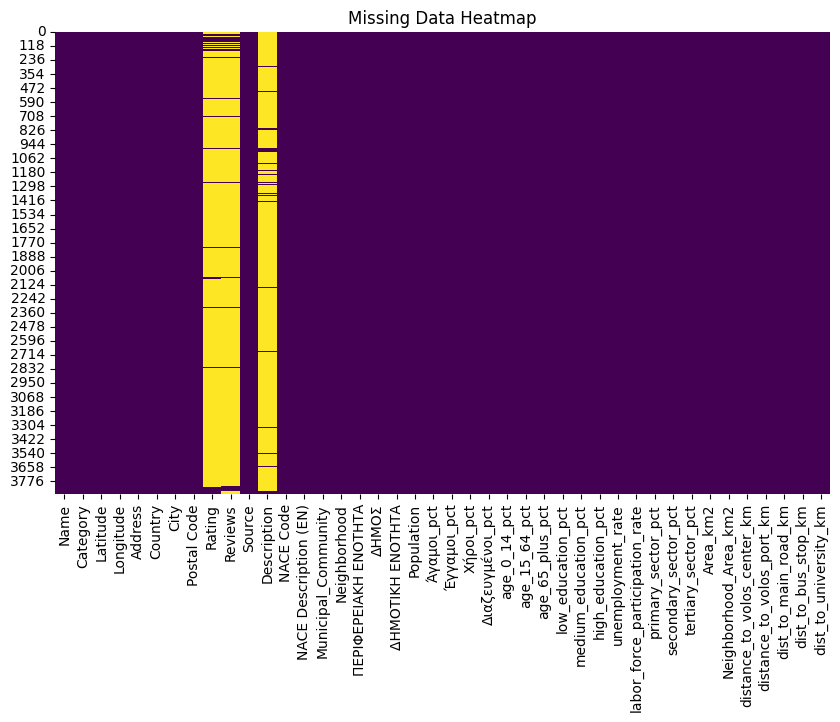
\includegraphics[scale=0.45]{figures/heatmap_missing.png}
    \centering
    \caption{Missing Data Heatmap}
    \label{fig:heatmap_missing}
\end{figure}



%========================================
%========================================
%========================================
\section{Proxy Ground Truths}
\label{venn_diagrams}


This appendix contains information about the procedure of creating the proxy ground truths. Below we present some indicative Venn diagrams of the agreement count between the three different proxy truth creation methods. Not every single one will be shown since their total number is 306 (1 per NACE class).


\begin{figure}[h]
    \centering
    \begin{minipage}[b]{0.47\textwidth}
        \centering
        
\includegraphics[height=5cm]{figures/venn_nace_47_25.png}
        \caption{Venn Diagram for NACE Class 47.25 (Partial Similarity)}
        \label{fig:venn_nace_47_25}
    \end{minipage}
    \hfill
    \begin{minipage}[b]{0.47\textwidth}
        \centering
        
\includegraphics[height=5cm]{figures/venn_nace_28_49.png}
        \caption{Venn Diagram for NACE Class 28.49 (Perfect Similarity)}
        \label{fig:venn_nace_28_49}
    \end{minipage}
\end{figure}

